\documentclass{beamer}

\usepackage{graphicx}
\usepackage{hyperref}
\usepackage{tikz}

\usefonttheme{serif}
\usetikzlibrary{arrows}

\title{2 - Integrated Circuits, Memory, and Haskell}
\author{}
\date{}

\begin{document}

\frame{\titlepage}

\begin{frame}
  \frametitle{Agenda}
  \tableofcontents
\end{frame}

\section{Transistor refresher: the NOT gate}

\begin{frame}
  \frametitle{A gate for inverting a signal: NOT}
  \begin{figure}
    \centering
    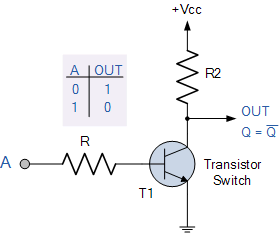
\includegraphics[width=0.5\textwidth]{res/not-gate.png}
  \end{figure}

  Build this on your breadboard!
\end{frame}

\section{Integrated circuits: AND and OR}

\begin{frame}
  \frametitle{Using integrated circuits}

  \begin{columns}
    \begin{column}{0.4\textwidth}
      \begin{figure}
          \centering
          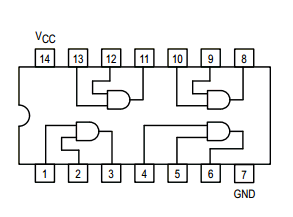
\includegraphics[width=\textwidth]{res/and-gate-ic.png}
      \end{figure}
    \end{column}
    \begin{column}{0.6\textwidth}
      \begin{itemize}
      \item
        The \emph{pinout} diagram for the 7408 AND gate. The OR gate is the
        same, only the ANDs are ORs.
      \item
        $V_{CC}$ needs to be connected to \emph{positive} and GND to
        \emph{negative}.  \alert{Important:} for an input to be considered as
        $0$ or \texttt{false} it must be connected to \emph{negative}!
      \item
        Test out the ICs on your breadboard by observing their output using an LED.
      \end{itemize}
    \end{column}
  \end{columns}
\end{frame}

\begin{frame}
  \frametitle{Computer memory foundations: an S-R latch}

  \url{https://www.youtube.com/watch?v=fpnE6UAfbtU} \\
  $1:27$ to $3:12$
\end{frame}

\begin{frame}
  \frametitle{Remember all that?}

  Now let's build an S-R latch using a transistor-based NOT gate and integrated
  circuit-based AND and OR gates!

  \begin{figure}
    \centering
    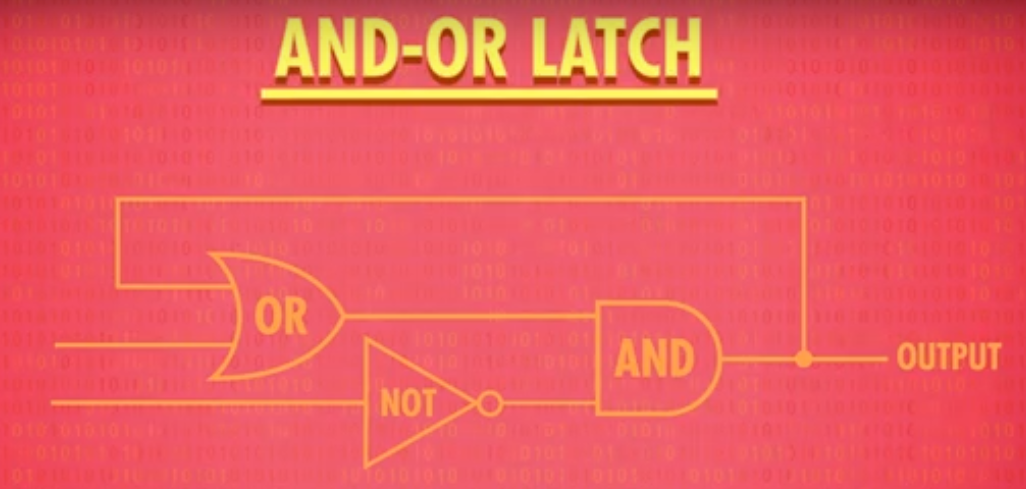
\includegraphics[width=0.7\textwidth]{res/and-or-latch.png}
  \end{figure}
\end{frame}

\begin{frame}
  \frametitle{Haskell}
%% Add: functions, and basic haskell types, really just lists and ints


  \begin{figure}
    \centering
    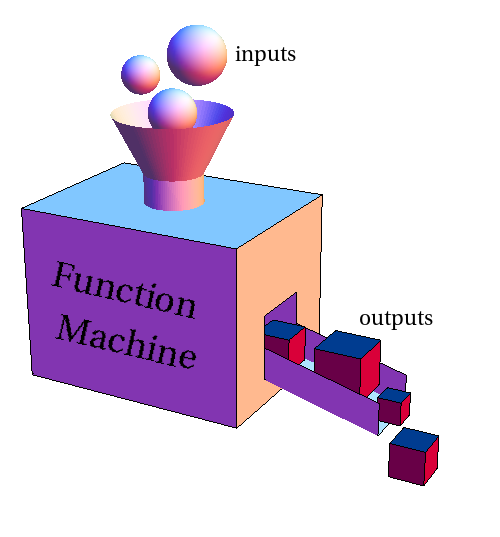
\includegraphics[width=0.5\textwidth]{res/function-machine.png}
  \end{figure}
\end{frame}

\begin{frame}
  \frametitle{Define all things}

  This is a simple definition, which gives a name to the \emph{expression} $25$.

  Elsewhere in a file, we can now write \texttt{age} instead of the literal
  number $25$; they are now synonyms.

  \begin{figure}
    \centering
    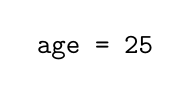
\begin{tikzpicture}
      \node at (0, 0) (f) {\texttt{age = 25}};
    \end{tikzpicture}
  \end{figure}

  \pause
  All definitions are set in stone. You can't change the meaning of something
  after you define it!

  We call \texttt{age} in this context a \alert{binding} and say that
  ``\texttt{age} is \emph{bound to} $25$.''

  The right-hand side of the definition is also called the \emph{body}.
\end{frame}

\begin{frame}
  \frametitle{Parametric!}

  A definition can take \emph{parameters}, in which case it defines a
  \emph{function}.

  % Functions are the most basic building blocks of \emph{functional programming}.

  \begin{figure}
    \centering
    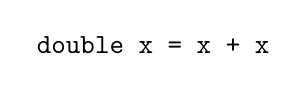
\begin{tikzpicture}
      \node at (0, 0) (f) {\texttt{double x = x + x}};
    \end{tikzpicture}
  \end{figure}

  \begin{itemize}
  \item
    Elsewhere in the file, if we write \texttt{double 25}, then that's the same
    thing as writing \texttt{25 + 25}, because definitions are like synonyms.
  \pause
  \item
    In this case, \texttt{double} is the binding, and \texttt{x} is a
    \alert{parameter}. Parameters refer to the \emph{input} of the function.

  \pause
  \item
    The output, on the other hand, is the body, and depends on the input.
  \end{itemize}
\end{frame}

\begin{frame}
  \frametitle{What type of function?}

  In Haskell, every expression has a \alert{type}.

  \begin{figure}
    \centering
    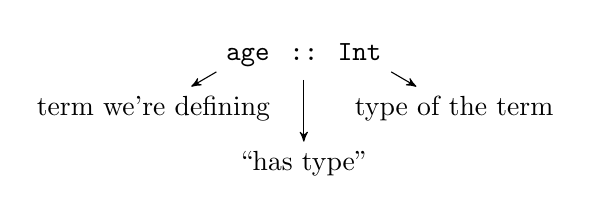
\begin{tikzpicture}[->, >=stealth']
    \path
    (0, 0)
    node (f) {\strut\texttt{age}}
    (f.east) node[anchor=west, baseline=f.base] (h) {\strut\texttt{::}}
    (h.east) node[anchor=west, baseline=f.base] (e) {\strut\texttt{Int}};
    \draw
    (f) ++(-1.2, -0.7) node (ex1) {term we're defining}
    (f) -- (ex1);
    \draw
    (h) ++(0, -1.4) node (ex2) {``has type''}
    (h) -- (ex2);
    \draw
    (e) ++(1.2, -0.7) node (ex3) {type of the term}
    (e) -- (ex3);
    \end{tikzpicture}
  \end{figure}
\end{frame}

\end{document}
